\subsection{Reducing the coboundary matrix}

The reduction by killing method (clearing) was found to be utilised to a much greater degree when using the cohomology (instead of the homology) of Vietoris-Rips filtrations. \textcite{de2011dualities} first published this cohomology algorithm; however, it compares the use of cohomology to the standard algorithm without clearing and thus his results may artificially bloat the effectiveness of this speed-up.

There are two main observations to understand this speed-up:
\begin{enumerate}
  \item the persistent barcodes from homology and cohomology are identical; and
  \item computing persistent barcodes on cohomology allows for more clearing.
\end{enumerate}

We have already seen that the persistent barcodes for homology and cohomology coincide (see Lemma \ref{lem:hom-cohom-barcodes-equiv}).

Let $\mathbb K = \{K_i\}_{i=0}^n$ be a maximal filtered simplicial complex and let $\sigma_1, \ldots, \sigma_n$ be the induced simplex ordering. The \emph{coboundary matrix} of $\mathbb K$ is defined by
\[ 
  \delta[i, j] = 
  \begin{cases}
    1 & \text{if $\sigma_{n+1-i}$ is a cofacet of $\sigma_{n+1-j}$}, \\
    0 & \text{otherwise}.
  \end{cases} 
\]
$\delta$ is simply the \emph{anti-transpose} (flip over the anti-diagonal) of the boundary matrix $\partial$, and we can construct it in the same time. We note that the basis for this matrix are the \emph{cochains} of the simplicial cochain complex, and thus mapping between the barcodes from persistent cohomology and persistent homology is just reversing the ordering of our basis (and mapping barcodes of the form $(\infty, i)$ to the form $(j, \infty)$ appropriately).

We now argue that cohomology allows for more clearing. In fact, this is not true for the general case. It is the properties of the Vietoris-Rips filtration that allow for more clearing. 

The clearing optimisation (\textsc{SSR}) sets a column $R_i$ to $\bm 0$ if $i$ is the pivot index of another column $R_j$. In terms of persistent barcodes, $R_i$ is a \emph{birth column} and $R_j$ is the \emph{death column}. It has already been noted that $\dim(\sigma_i) = \dim(\sigma_j) - 1$. Thus to clear the column of a $k$-simplex, we must reduce the column of a $(k+1)$-simplex. Conversely, in cohomology, clearing the column a $k$-simplex requires the reduction of the column of a $(k-1)$-simplex. Thus, as 

For Vietoris-Rips filtrations, the degree we calculate persistent homology to is often small, and there are often many more $(d+1)$-simplices than simplices of lower dimension. In homology, clearing is not available for the $(d+1)$-simplices. However, in cohomology, clearing is not available for the $0$-simplices. As there are (often) more $(d+1)$-simplices then $0$-simplices, cohomology allows for more clearing for Vietoris-Rips filtrations.

We refer to the algorithm utilising sparse matrix representation, reduction by killing, and the cohomology boundary matrix as \textsc{SSRCoh}. 

An experiment was conducted comparing \textsc{SSR} and \textsc{SSRCoh}. A Vietoris-Rips filtration was constructed from a sample of 1000 points from the noisy unit circle (radius fluctuation $\pm 0.05$), as in the last experiment. We run both algorithms from $\varepsilon = 0.01$ to $\varepsilon = 0.06$. Figure \ref{fig:speedsup-3v4} shows the result of this experiment, and empirically verifies our predicted speed-up.

\begin{figure}
  \makebox[\textwidth][c]{
  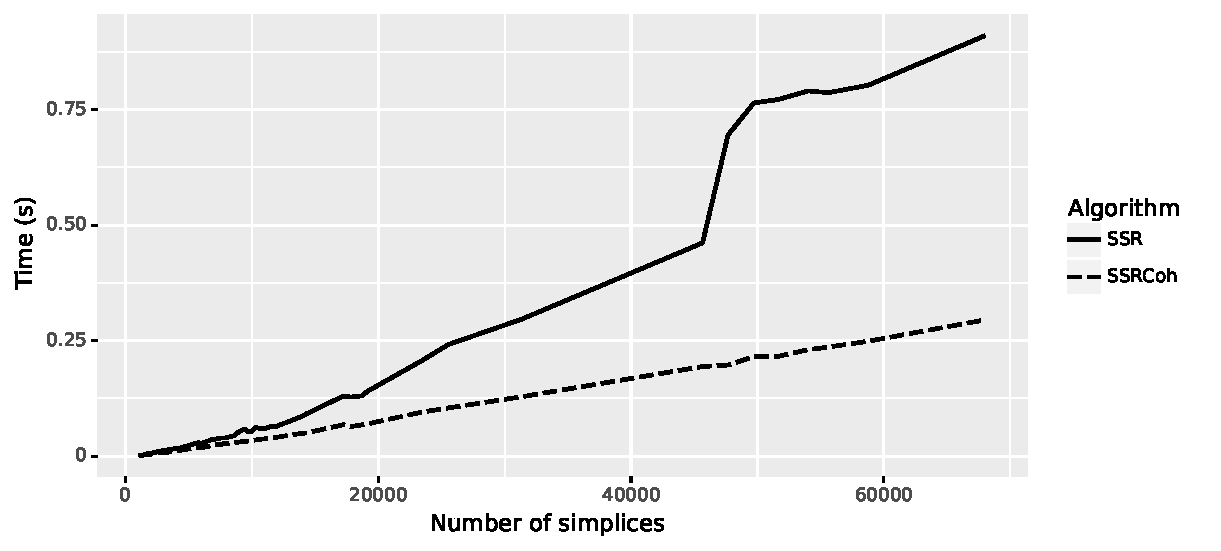
\includegraphics[width=1.2\textwidth]{content/4-comp-top/images/2-3v4-circ-compute}
  }
  \caption{A plot of the running time of \textsc{SSR} and \textsc{SSRCoh} algorithms on a Vietoris-Rips complex constructed from a noisy unit circle.}
  \label{fig:speedsup-3v4}
\end{figure}
